\section{欧拉回路与哈密尔顿回路}

\subsection{欧拉通路(Euler Trail) / 欧拉回路(Euler Circuit)}

Konigsberg被一条河流分成4块区域,有7座桥把这4块区域连接了起来。镇上的人们想弄明白是否可能从某块区域出发,不重复地经过所有桥并且回到出发点。

\begin{figure}[H]
	\centering
	\begin{tikzpicture}[x=10cm, y=9.19cm]
		%water
		\filldraw[water] (0, 0) -- (0, 1) -- (1, 1) -- (1, 0) -- cycle;

		%bridge top 1
		\filldraw[bridge] ($(0, 1) + (0.329, -0.300)$) --
		($(0, 1) + (0.423, -0.301)$) -- ($(0, 1) + (0.399, -0.399)$) --
		($(0, 1) + (0.328, -0.404)$) -- cycle;
		\draw[contour] ($(0, 1) + (0.423, -0.301)$) -- ($(0, 1) + (0.399, -0.399)$)
		($(0, 1) + (0.328, -0.404)$) -- ($(0, 1) + (0.329, -0.300)$);

		%bridge top 2
		\filldraw[bridge] ($(0, 1) + (0.532, -0.302)$) --
		($(0, 1) + (0.558, -0.310)$) -- ($(0, 1) + (0.591, -0.338)$) --
		($(0, 1) + (0.609, -0.404)$) -- ($(0, 1) + (0.549, -0.388)$) --
		cycle;
		\draw[contour] ($(0, 1) + (0.591, -0.338)$) -- ($(0, 1) + (0.609, -0.404)$)
		($(0, 1) + (0.532, -0.302)$) -- ($(0, 1) + (0.549, -0.388)$);

		%bridge top 3
		\filldraw[bridge] ($(0, 1) + (0.635, -0.328)$) --
		($(0, 1) + (0.656, -0.304)$) -- ($(0, 1) + (0.669, -0.276)$) --
		($(0, 1) + (0.796, -0.364)$) --
		($(0, 1) + (0.776, -0.396)$) -- ($(0, 1) + (0.762, -0.420)$) -- cycle;
		\draw[contour] ($(0, 1) + (0.635, -0.328)$) -- ($(0, 1) + (0.762, -0.420)$)
		($(0, 1) + (0.669, -0.276)$) -- ($(0, 1) + (0.796, -0.364)$);

		%bridge middle right
		\filldraw[bridge] ($(0, 1) + (0.658, -0.590)$) --
		($(0, 1) + (0.668, -0.546)$) -- ($(0, 1) + (0.778, -0.524)$) --
		($(0, 1) + (0.792, -0.554)$) -- ($(0, 1) + (0.796, -0.590)$) --cycle;
		\draw[contour] ($(0, 1) + (0.668, -0.546)$) -- ($(0, 1) + (0.778, -0.524)$)
		($(0, 1) + (0.658, -0.590)$) -- ($(0, 1) + (0.796, -0.590)$);

		%bridge bottom 1
		\filldraw[bridge] ($(0, 1) + (0.350, -0.826)$) --
		($(0, 1) + (0.410, -0.804)$) -- ($(0, 1) + (0.422, -0.794)$) --
		($(0, 1) + (0.412, -0.708)$) -- ($(0, 1) + (0.372, -0.702)$) --
		($(0, 1) + (0.336, -0.695)$) -- cycle;
		\draw[contour] ($(0, 1) + (0.422, -0.794)$) -- ($(0, 1) + (0.412, -0.708)$)
		($(0, 1) + (0.350, -0.826)$) -- ($(0, 1) + (0.336, -0.695)$);

		%bridge bottom 2
		\filldraw[bridge] ($(0, 1) + (0.596, -0.700)$) --
		($(0, 1) + (0.535, -0.708)$) -- ($(0, 1) + (0.523, -0.784)$) --
		($(0, 1) + (0.581, -0.777)$) -- cycle;
		\draw[contour] ($(0, 1) + (0.535, -0.708)$) -- ($(0, 1) + (0.523, -0.784)$)
		($(0, 1) + (0.596, -0.700)$) -- ($(0, 1) + (0.581, -0.777)$);

		%bridge bottom 3
		\filldraw[bridge] ($(0, 1) + (0.581, -0.777)$) --
		($(0, 1) + (0.660, -0.862)$) -- ($(0, 1) + (0.858, -0.717)$) --
		($(0, 1) + (0.837, -0.702)$) -- ($(0, 1) + (0.826, -0.688)$) --
		($(0, 1) + (0.785, -0.668)$) -- cycle;
		\draw[contour] ($(0, 1) + (0.581, -0.777)$) -- ($(0, 1) + (0.785, -0.668)$)
		($(0, 1) + (0.660, -0.862)$) -- ($(0, 1) + (0.858, -0.717)$);

		%land top
		\filldraw[land] (0, 1) --
		($(0, 1) + (0, -0.287)$) -- ($(0, 1) + (0.080, -0.287)$) --
		($(0, 1) + (0.161, -0.281)$) -- ($(0, 1) + (0.178, -0.273)$) --
		($(0, 1) + (0.257, -0.289)$) -- ($(0, 1) + (0.280, -0.287)$) --
		($(0, 1) + (0.329, -0.300)$) -- ($(0, 1) + (0.423, -0.301)$) --
		($(0, 1) + (0.532, -0.302)$) -- ($(0, 1) + (0.558, -0.310)$) --
		($(0, 1) + (0.591, -0.338)$) -- ($(0, 1) + (0.635, -0.328)$) --
		($(0, 1) + (0.656, -0.304)$) -- ($(0, 1) + (0.669, -0.276)$) --
		($(0, 1) + (0.720, -0.246)$) -- ($(0, 1) + (0.741, -0.233)$) --
		($(0, 1) + (0.780, -0.210)$) -- ($(0, 1) + (0.824, -0.206)$) --
		($(0, 1) + (0.874, -0.178)$) -- ($(0, 1) + (0.931, -0.169)$) --
		($(0, 1) + (0.969, -0.161)$) -- ($(1, 1) + (0, -0.149)$) --
		(1, 1) -- cycle;
		\draw[contour] ($(0, 1) + (0, -0.287)$) -- ($(0, 1) + (0.080, -0.287)$) --
		($(0, 1) + (0.161, -0.281)$) -- ($(0, 1) + (0.178, -0.273)$) --
		($(0, 1) + (0.257, -0.289)$) -- ($(0, 1) + (0.280, -0.287)$) --
		($(0, 1) + (0.329, -0.300)$) -- ($(0, 1) + (0.423, -0.301)$) --
		($(0, 1) + (0.532, -0.302)$) -- ($(0, 1) + (0.558, -0.310)$) --
		($(0, 1) + (0.591, -0.338)$) -- ($(0, 1) + (0.635, -0.328)$) --
		($(0, 1) + (0.656, -0.304)$) -- ($(0, 1) + (0.669, -0.276)$) --
		($(0, 1) + (0.720, -0.246)$) -- ($(0, 1) + (0.741, -0.233)$) --
		($(0, 1) + (0.780, -0.210)$) -- ($(0, 1) + (0.824, -0.206)$) --
		($(0, 1) + (0.874, -0.178)$) -- ($(0, 1) + (0.931, -0.169)$) --
		($(0, 1) + (0.969, -0.161)$) -- ($(1, 1) + (0, -0.149)$);

		%land bottom
		\filldraw[land] ($(0, 1) + (0, -0.890)$) -- ($(0, 1) + (0.067, -0.880)$) --
		($(0, 1) + (0.067, -0.880)$) -- ($(0, 1) + (0.085, -0.860)$) --
		($(0, 1) + (0.111, -0.858)$) -- ($(0, 1) + (0.139, -0.849)$) --
		($(0, 1) + (0.161, -0.860)$) -- ($(0, 1) + (0.212, -0.847)$) --
		($(0, 1) + (0.242, -0.830)$) -- ($(0, 1) + (0.350, -0.826)$) --
		($(0, 1) + (0.410, -0.804)$) -- ($(0, 1) + (0.422, -0.794)$) --
		($(0, 1) + (0.450, -0.784)$) -- ($(0, 1) + (0.523, -0.784)$) --
		($(0, 1) + (0.581, -0.777)$) -- ($(0, 1) + (0.660, -0.862)$) --
		($(0, 1) + (0.672, -0.882)$) -- ($(0, 1) + (0.679, -0.924)$) --
		($(0, 1) + (0.698, -0.968)$) -- ($(0, 1) + (0.714, -0.990)$) --
		(0.718, 0) -- (0, 0) -- cycle;
		\draw[contour] ($(0, 1) + (0, -0.890)$) -- ($(0, 1) + (0.067, -0.880)$) --
		($(0, 1) + (0.067, -0.880)$) -- ($(0, 1) + (0.085, -0.860)$) --
		($(0, 1) + (0.111, -0.858)$) -- ($(0, 1) + (0.139, -0.849)$) --
		($(0, 1) + (0.161, -0.860)$) -- ($(0, 1) + (0.212, -0.847)$) --
		($(0, 1) + (0.242, -0.830)$) -- ($(0, 1) + (0.350, -0.826)$) --
		($(0, 1) + (0.410, -0.804)$) -- ($(0, 1) + (0.422, -0.794)$) --
		($(0, 1) + (0.450, -0.784)$) -- ($(0, 1) + (0.523, -0.784)$) --
		($(0, 1) + (0.581, -0.777)$) -- ($(0, 1) + (0.660, -0.862)$) --
		($(0, 1) + (0.672, -0.882)$) -- ($(0, 1) + (0.679, -0.924)$) --
		($(0, 1) + (0.698, -0.968)$) -- ($(0, 1) + (0.714, -0.990)$) --
		(0.718, 0);

		%land right
		\filldraw[land] (1, 0) -- ($(0, 1) + (0.978, -0.975)$) --
		($(0, 1) + (0.954, -0.908)$) -- ($(0, 1) + (0.921, -0.829)$) --
		($(0, 1) + (0.900, -0.810)$) -- ($(0, 1) + (0.880, -0.775)$) --
		($(0, 1) + (0.858, -0.717)$) -- ($(0, 1) + (0.837, -0.702)$) --
		($(0, 1) + (0.826, -0.688)$) -- ($(0, 1) + (0.785, -0.668)$) --
		($(0, 1) + (0.796, -0.623)$) -- ($(0, 1) + (0.796, -0.590)$) --
		($(0, 1) + (0.792, -0.554)$) -- ($(0, 1) + (0.778, -0.524)$) --
		($(0, 1) + (0.764, -0.466)$) -- ($(0, 1) + (0.762, -0.420)$) --
		($(0, 1) + (0.776, -0.396)$) -- ($(0, 1) + (0.796, -0.364)$) --
		($(0, 1) + (0.838, -0.368)$) -- ($(0, 1) + (0.864, -0.380)$) --
		($(0, 1) + (0.910, -0.384)$) -- ($(0, 1) + (0.946, -0.392)$) --
		($(0, 1) + (0.971, -0.394)$) -- ($(0, 1) + (1, -0.414)$) -- cycle;
		\draw[contour] (1, 0) -- ($(0, 1) + (0.978, -0.975)$) --
		($(0, 1) + (0.954, -0.908)$) -- ($(0, 1) + (0.921, -0.829)$) --
		($(0, 1) + (0.900, -0.810)$) -- ($(0, 1) + (0.880, -0.775)$) --
		($(0, 1) + (0.858, -0.717)$) -- ($(0, 1) + (0.837, -0.702)$) --
		($(0, 1) + (0.826, -0.688)$) -- ($(0, 1) + (0.785, -0.668)$) --
		($(0, 1) + (0.796, -0.623)$) -- ($(0, 1) + (0.796, -0.590)$) --
		($(0, 1) + (0.792, -0.554)$) -- ($(0, 1) + (0.778, -0.524)$) --
		($(0, 1) + (0.764, -0.466)$) -- ($(0, 1) + (0.762, -0.420)$) --
		($(0, 1) + (0.776, -0.396)$) -- ($(0, 1) + (0.796, -0.364)$) --
		($(0, 1) + (0.838, -0.368)$) -- ($(0, 1) + (0.864, -0.380)$) --
		($(0, 1) + (0.910, -0.384)$) -- ($(0, 1) + (0.946, -0.392)$) --
		($(0, 1) + (0.971, -0.394)$) -- ($(0, 1) + (1, -0.414)$);

		%island
		\filldraw[land] ($(0, 1) + (0.241, -0.622)$) -- ($(0, 1) + (0.235, -0.587)$) --
		($(0, 1) + (0.240, -0.540)$) -- ($(0, 1) + (0.249, -0.524)$) --
		($(0, 1) + (0.252, -0.498)$) -- ($(0, 1) + (0.266, -0.482)$) --
		($(0, 1) + (0.271, -0.462)$) -- ($(0, 1) + (0.288, -0.454)$) --
		($(0, 1) + (0.300, -0.434)$) -- ($(0, 1) + (0.308, -0.418)$) --
		($(0, 1) + (0.320, -0.412)$) -- ($(0, 1) + (0.328, -0.404)$) --
		($(0, 1) + (0.399, -0.399)$) -- ($(0, 1) + (0.453, -0.393)$) --
		($(0, 1) + (0.518, -0.386)$) -- ($(0, 1) + (0.549, -0.388)$) --
		($(0, 1) + (0.609, -0.404)$) -- ($(0, 1) + (0.624, -0.410)$) --
		($(0, 1) + (0.644, -0.438)$) -- ($(0, 1) + (0.663, -0.486)$) --
		($(0, 1) + (0.670, -0.519)$) -- ($(0, 1) + (0.668, -0.546)$) --
		($(0, 1) + (0.658, -0.590)$) -- ($(0, 1) + (0.648, -0.612)$) --
		($(0, 1) + (0.636, -0.648)$) -- ($(0, 1) + (0.633, -0.666)$) --
		($(0, 1) + (0.617, -0.677)$) -- ($(0, 1) + (0.596, -0.700)$) --
		($(0, 1) + (0.535, -0.708)$) -- ($(0, 1) + (0.500, -0.709)$) --
		($(0, 1) + (0.457, -0.717)$) -- ($(0, 1) + (0.412, -0.708)$) --
		($(0, 1) + (0.372, -0.702)$) -- ($(0, 1) + (0.336, -0.695)$) --
		($(0, 1) + (0.291, -0.679)$) -- ($(0, 1) + (0.268, -0.652)$) --
		cycle;
		\draw[contour] ($(0, 1) + (0.241, -0.622)$) -- ($(0, 1) + (0.235, -0.587)$) --
		($(0, 1) + (0.240, -0.540)$) -- ($(0, 1) + (0.249, -0.524)$) --
		($(0, 1) + (0.252, -0.498)$) -- ($(0, 1) + (0.266, -0.482)$) --
		($(0, 1) + (0.271, -0.462)$) -- ($(0, 1) + (0.288, -0.454)$) --
		($(0, 1) + (0.300, -0.434)$) -- ($(0, 1) + (0.308, -0.418)$) --
		($(0, 1) + (0.320, -0.412)$) -- ($(0, 1) + (0.328, -0.404)$) --
		($(0, 1) + (0.399, -0.399)$) -- ($(0, 1) + (0.453, -0.393)$) --
		($(0, 1) + (0.518, -0.386)$) -- ($(0, 1) + (0.549, -0.388)$) --
		($(0, 1) + (0.609, -0.404)$) -- ($(0, 1) + (0.624, -0.410)$) --
		($(0, 1) + (0.644, -0.438)$) -- ($(0, 1) + (0.663, -0.486)$) --
		($(0, 1) + (0.670, -0.519)$) -- ($(0, 1) + (0.668, -0.546)$) --
		($(0, 1) + (0.658, -0.590)$) -- ($(0, 1) + (0.648, -0.612)$) --
		($(0, 1) + (0.636, -0.648)$) -- ($(0, 1) + (0.633, -0.666)$) --
		($(0, 1) + (0.617, -0.677)$) -- ($(0, 1) + (0.596, -0.700)$) --
		($(0, 1) + (0.535, -0.708)$) -- ($(0, 1) + (0.500, -0.709)$) --
		($(0, 1) + (0.457, -0.717)$) -- ($(0, 1) + (0.412, -0.708)$) --
		($(0, 1) + (0.372, -0.702)$) -- ($(0, 1) + (0.336, -0.695)$) --
		($(0, 1) + (0.291, -0.679)$) -- ($(0, 1) + (0.268, -0.652)$) --
		($(0, 1) + (0.241, -0.622)$);
	\end{tikzpicture}
	\caption{哥尼斯堡七桥问题}
\end{figure}

这个问题可以用图进行描述,顶点用于表示4块区域,边用于表示连接两个区域的桥。这样问题就转化成了能否不重复地一笔画完所有的边,即图是否存在欧拉回路。

\begin{figure}[H]
	\centering
	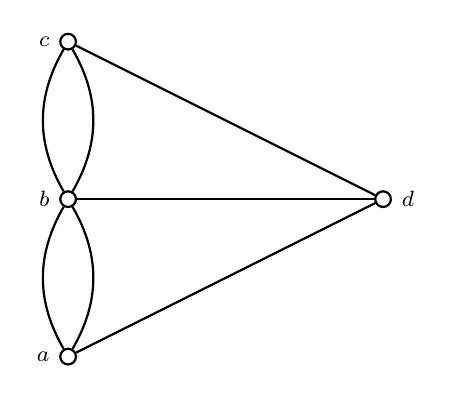
\begin{tikzpicture}
		[lineDecorate/.style={-,thick},
			nodeDecorate/.style={shape=circle,inner sep=2pt,draw,thick}]
		\foreach \nodename/\x/\y/\direction/\navigate in {
				a/0/0/left/west, b/0/2/left/west, c/0/4/left/west, d/4/2/right/east}
			{
				\node (\nodename) at (\x,\y) [nodeDecorate] {};
				\node [\direction] at (\nodename.\navigate) {\footnotesize$\nodename$};
			}
		\path
		\foreach \startnode/\endnode in {a/d, b/d, c/d}
			{
				(\startnode) edge[lineDecorate] node {} (\endnode)
			}
		\foreach \startnode/\endnode in {a/b, b/c, c/b, b/a}
			{
				(\startnode) edge[lineDecorate,bend left] node {} (\endnode)
			};
	\end{tikzpicture}
\end{figure}

1736年,29岁的欧拉向圣彼得堡科学院递交了关于哥尼斯堡七桥问题的论文。在解答问题的同时,开创了数学的一个新的分支——图论与几何拓扑,也由此展开了数学史上的新历程。\\

七桥问题提出后,很多人对此很感兴趣,纷纷进行试验,但在相当长的时间里,始终未能解决。欧拉通过对七桥问题的研究,不仅圆满地回答了哥尼斯堡居民提出的问题,而且得到并证明了更为广泛的有关一笔画的三条结论。\\

欧拉通路与欧拉回路的区别在于,欧拉通路需要经过图中所有边正好一次,而欧拉回路则需要经过图中所有边正好一次并最终回到出发点。

\begin{tcolorbox}
	\mybox{Exercise}
	判断在一个有度为奇数的顶点的图中是否存在一条欧拉回路。\\
	假设图G存在欧拉回路,令v为回路中的第一个顶点。从第一个顶点出发离开会使当前顶点的度增加1。\\
	经过回路中的中间顶点时,每个顶点的度都会增加2,一个入度,一个出度。\\
	最后一条边必须回到第一个顶点v,这样会使第一个顶点v的度增加1。\\
	因为每一个顶点都有可能作为出发点,因此只有顶点度都为偶数的图才有可能存在欧拉回路。
\end{tcolorbox}

一个连通图存在欧拉通路但无欧拉回路,当且仅当它恰好拥有2个度为奇数的顶点。

\begin{figure}[H]
	\centering
	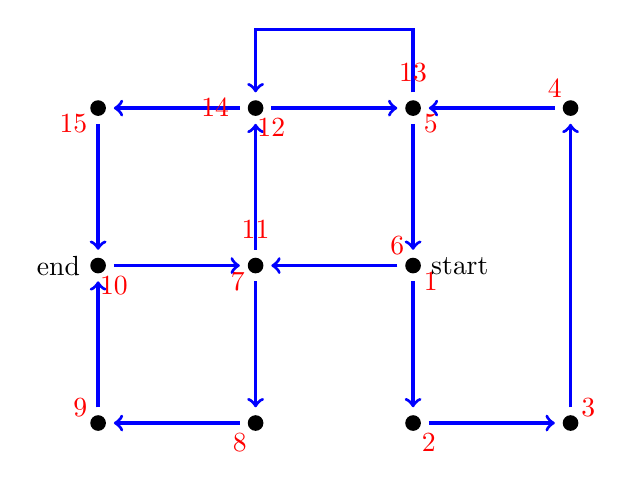
\begin{tikzpicture}
		\node[black, fill=black, circle, inner sep=2pt] at (0,0){};
		\node[black, fill=black, circle, inner sep=2pt, label=left:end] at (0,2){};
		\node[black, fill=black, circle, inner sep=2pt] at (0,4){};
		\node[black, fill=black, circle, inner sep=2pt] at (2,0){};
		\node[black, fill=black, circle, inner sep=2pt] at (2,2){};
		\node[black, fill=black, circle, inner sep=2pt] at (2,4){};
		\node[black, fill=black, circle, inner sep=2pt] at (4,0){};
		\node[black, fill=black, circle, inner sep=2pt, label=right:start] at (4,2){};
		\node[black, fill=black, circle, inner sep=2pt] at (4,4){};
		\node[black, fill=black, circle, inner sep=2pt] at (6,0){};
		\node[black, fill=black, circle, inner sep=2pt] at (6,4){};

		\draw[blue, very thick, ->] (4,1.8) node[right, red]{1} -- (4,0.2);
		\draw[blue, very thick, ->] (4.2,0) node[below, red]{2} -- (5.8,0);
		\draw[blue, very thick, ->] (6,0.2) node[right, red]{3} -- (6,3.8);
		\draw[blue, very thick, ->] (5.8,4) node[above, red]{4} -- (4.2,4);
		\draw[blue, very thick, ->] (4,3.8) node[right, red]{5} -- (4,2.2);
		\draw[blue, very thick, ->] (3.8,2) node[above, red]{6} -- (2.2,2);
		\draw[blue, very thick, ->] (2,1.8) node[left, red]{7} -- (2,0.2);
		\draw[blue, very thick, ->] (1.8,0) node[below, red]{8} -- (0.2,0);
		\draw[blue, very thick, ->] (0,0.2) node[left, red]{9} -- (0,1.8);
		\draw[blue, very thick, ->] (0.2,2) node[below, red]{10} -- (1.8,2);
		\draw[blue, very thick, ->] (2,2.2) node[above, red]{11} -- (2,3.8);
		\draw[blue, very thick, ->] (2.2,4) node[below, red]{12} -- (3.8,4);
		\draw[blue, very thick, ->] (4,4.2) node[above, red]{13} -- (4,5) -- (2,5) -- (2,4.2);
		\draw[blue, very thick, ->] (1.8,4) node[left, red]{14} -- (0.2,4);
		\draw[blue, very thick, ->] (0,3.8) node[left, red]{15} -- (0,2.2);
	\end{tikzpicture}
	\caption{欧拉通路}
\end{figure}